\documentclass[11pt]{article}
\usepackage[T1]{fontenc}
\usepackage[utf8]{inputenc}
\usepackage{lmodern}
\usepackage[a4paper,margin=27mm,headheight=15pt]{geometry}
\usepackage{amsmath,amssymb,amsthm,mathtools}
\usepackage{microtype}
\usepackage{booktabs,longtable,array,enumitem}
\usepackage{xcolor,graphicx}
\usepackage{fancyhdr}
\usepackage[hidelinks]{hyperref}
\usepackage{listings}
\definecolor{ink}{HTML}{15364A}
\definecolor{accent}{HTML}{126C75}
\definecolor{pale}{HTML}{EDF4F6}
\hypersetup{pdftitle={A quantitative Jordan curve theorem in intuitionistic primitive recursive arithmetic},
 pdfauthor={Research prepared for Vladimir Reshetnikov},
 pdfsubject={Constructive topology; primitive recursive arithmetic; Lean formalization plan}}
\pagestyle{fancy}
\fancyhf{}
\fancyhead[L]{\small\color{ink}Constructive Jordan theorem in iPRA}
\fancyhead[R]{\small\thepage}
\renewcommand{\headrulewidth}{0.3pt}
\setlength{\parskip}{4pt}
\setlength{\parindent}{0pt}
\setlist{itemsep=3pt,topsep=5pt}
\newtheorem{theorem}{Theorem}[section]
\newtheorem{lemma}[theorem]{Lemma}
\newtheorem{proposition}[theorem]{Proposition}
\newtheorem{corollary}[theorem]{Corollary}
\theoremstyle{definition}
\newtheorem{definition}[theorem]{Definition}
\newtheorem{remark}[theorem]{Remark}
\newcommand{\N}{\mathbb N}
\newcommand{\Q}{\mathbb Q}
\newcommand{\R}{\mathbb R}
\newcommand{\T}{\mathbb T}
\newcommand{\F}{\mathbb F_2}
\newcommand{\ipra}{\mathsf{iPRA}}
\newcommand{\norm}[1]{\left\lVert #1\right\rVert_\infty}
\newcommand{\dist}{\operatorname{dist}}
\newcommand{\parity}{\operatorname{par}}
\newcommand{\Reg}{\operatorname{Reg}}
\newcommand{\xor}{\mathbin{\oplus}}
\newcommand{\ceil}[1]{\left\lceil #1\right\rceil}
\newcommand{\code}[1]{\texttt{\small #1}}
\newcommand{\repo}{\texttt{ConciseIPRA}}
\newcommand{\eps}{\varepsilon}
\lstset{basicstyle=\ttfamily\footnotesize,breaklines=true,columns=fullflexible,
 frame=single,rulecolor=\color{pale},backgroundcolor=\color{pale},
 keepspaces=true,showstringspaces=false}
\begin{document}
\begin{titlepage}
\vspace*{12mm}
{\large\color{accent}CONSTRUCTIVE TOPOLOGY / PROOF THEORY\par}
\vspace{9mm}
{\huge\bfseries\color{ink}A quantitative Jordan curve theorem\par}
\vspace{4mm}
{\LARGE in intuitionistic primitive recursive arithmetic\par}
\vspace{8mm}
{\large Finite parity, bounded routing, and a constructive common boundary\par}
\vspace{13mm}
{\large Prepared for Vladimir Reshetnikov\par}
{15 November 2026\par}
\vspace{10mm}
\begin{abstract}
We give a complete constructive proof of a quantitative Jordan curve theorem
for a circle embedding supplied by primitive recursive rational names, a
forward continuity modulus, and a positive inverse separation modulus.
For every point with certified positive distance from the curve, a finite
calculation returns its inside/outside bit. Equal bits yield a polygonal
connecting path with an explicit positive clearance. Both bits occur
arbitrarily near every curve point, with primitive recursive witnesses.
Every uniformly continuous path between different bits has approximate
intersections with the curve at every requested precision.

The proof uses rational arithmetic and crossing parity, not analytic winding
numbers. A bounded honeycomb search either finds a route or constructs a
boundary cycle whose parity factors through the original parameter circle.
A finite square-coloring argument supplies both sides. All search bounds
and the quantifier-free induction discipline are made explicit.
The first-order conclusion is a schema for fixed primitive recursive
presentations, not a quantification over arbitrary real functions.
\end{abstract}
\vfill
\colorbox{pale}{\parbox{\dimexpr\textwidth-2\fboxsep\relax}{
\textbf{Verification status.}
The human argument and its arithmetic interpretation are supplied in full.
The accompanying exact rational Python kernel was executed.
The Lean files are uncompiled implementation scaffolds and a detailed
completion plan; this package does not claim a completed Lean proof or an
already generated object-level iPRA derivation.}}
\end{titlepage}
\begingroup
\small
\setlength{\parskip}{0pt}
\tableofcontents
\endgroup
\newpage
\section{The theorem and its precise constructive meaning}\label{sec:statement}

\subsection{What is proved}

The usual Jordan theorem says that the complement of a simple closed plane
curve has exactly two connected components, one bounded and one unbounded,
and that the curve is their common boundary. In constructive arithmetic,
both the input and the conclusion must say what information is available.
In particular, a negative assertion that a point is not on the curve does
not supply a positive distance bound.

Our input is a quantitatively presented embedding
\[
 \gamma:\T\longrightarrow\R^2,\qquad \T=\R/\mathbb Z,
\]
where the circle distance is
\[
 d_\T(s,t)=\min(|s-t|,\,1-|s-t|)
 \quad(0\le s,t<1),
\]
and the plane uses the maximum norm. Rational coordinates, rational
parameters modulo one, and this norm make all finite computations exact.

\begin{definition}[Quantitative presentation]\label{def:presentation}
A presentation consists of a rational approximation routine
$G(q,n)\in\Q^2$, for $q\in\Q/\mathbb Z$, and nondecreasing functions
$U,V:\N\to\N$ with $U(k),V(k)\ge k+8$. Its associated curve has
\begin{align}
 \norm{G(q,n)-\gamma(q)}&\le 2^{-n},\label{eq:name}\\
 d_\T(s,t)\le 2^{-U(k)}
   &\ \Longrightarrow\
       \norm{\gamma(s)-\gamma(t)}\le 2^{-k},\label{eq:forward}\\
 d_\T(s,t)\ge 2^{-k}
   &\ \Longrightarrow\
       \norm{\gamma(s)-\gamma(t)}\ge 2^{-V(k)}.\label{eq:inverse}
\end{align}
All three routines are primitive recursive for an iPRA instance.
The second modulus is supplied data.
\end{definition}

The normalization of the moduli loses nothing: replace a modulus by the
maximum of its preceding values and $k+8$. The inverse condition is a
positive quantitative injectivity assertion. For rational $s,t$ it also
gives the usable implication
\[
 \norm{\gamma(s)-\gamma(t)}<2^{-V(k)}
 \ \Longrightarrow\ d_\T(s,t)<2^{-k};
\]
the comparison of the rational parameter distances is decidable.
The conditions extend to fast Cauchy parameter names by rational
approximation; the explicit padding used when the input assumptions
are stated only on rational parameters is given in
Section~\ref{sec:padding}.

Write $\Gamma$ for the image of the completed parameter circle.
An \emph{off-curve point} is a named point $x$ together with a natural
number $k_x$ certifying
\begin{equation}
 \norm{x-\gamma(t)}\ge 2^{-k_x}\quad\hbox{for every }t\in\T.
 \label{eq:off}
\end{equation}
The \emph{apartness complement} is the collection of points with such a
witness. A polygonal route has a finite list of vertices and a positive
rational lower bound for the distance of every one of its segments from
$\Gamma$. Its intermediate vertices can be rational even when its two
endpoints are named real points.

\begin{theorem}[Quantitative constructive Jordan theorem]\label{thm:main}
For a presentation as in Definition~\ref{def:presentation}, there are
primitive recursive procedures, relative to its fixed routines, with the
following properties.
\begin{enumerate}[label=\textnormal{(\arabic*)}]
\item \textbf{Classification.} Every off-curve point has a bit
$b_\Gamma(x)\in\{0,1\}$, independent of the chosen clearance certificate
and sufficiently accurate approximations. The bit is locally constant
on the apartness complement.
\item \textbf{Routing.} Given two off-curve points with equal bits, the
procedures return a polygonal route between them and a positive rational
clearance for that route.
\item \textbf{Separation.} A path with a supplied uniform continuity
modulus and positive clearance from $\Gamma$ has equal endpoint bits.
If instead its endpoints have different bits, then for every $n$ a
bounded calculation returns rational parameters $s,t$ such that
\[
       \norm{\alpha(s)-\gamma(t)}<2^{-n}.
\]
\item \textbf{Both sides.} Given a named parameter $t$ and $n$, the
procedures return rational points $a_0,a_1$ with explicit positive
clearances, with
\[
 b_\Gamma(a_0)=0,\qquad b_\Gamma(a_1)=1,\qquad
 \norm{a_i-\gamma(t)}<2^{-n}.
\]
\item \textbf{Size of the regions.} A primitive recursive bound $R$
for $\Gamma$ can be calculated. Every point with
$\norm{x}>R$ has bit zero. Thus the bit-one region is bounded and
inhabited, and the bit-zero region is unbounded and inhabited.
\item \textbf{Common boundary.} The image $\Gamma$ is exactly the set
of named points every neighborhood of which contains a rational
off-curve point of each bit. In the reverse direction a primitive recursive
circle name for a preimage is reconstructed from the point name.
\end{enumerate}
Consequently the apartness complement has exactly two classes under
the relation of being joined by a polygonal route with positive
clearance. Each class is open in the quantitative sense, and every
curve point is approached from both classes.
\end{theorem}

The term \emph{component} in this constructive conclusion has the explicitly
stated path-and-clearance meaning. We do not infer a uniform lower bound
from a merely pointwise claim that a continuous path misses the curve.
Nor do we replace the approximate intersection conclusion by the choice
of an exact zero or an exact crossing parameter. Those are different
selection assertions.

There is no rectifiability, differentiability, curvature, polygonality,
or supplied extension to a plane homeomorphism assumption. Classically,
continuous circle embeddings have forward and inverse moduli by
compactness. Here the moduli are part of the constructive presentation;
for the first-order iPRA claim they must be primitive recursive.

\subsection{How a first-order arithmetic theory speaks about these objects}
\label{sec:names}

iPRA has natural-number variables, function symbols for primitive recursive
functions, intuitionistic first-order logic, and quantifier-free induction.
It does not have a sort containing all real functions.
The preceding notation is an economical way to describe an
\emph{arithmetical theorem schema}.

Fix a finite collection of primitive recursive definitions for $G,U_0,V_0$
and, where needed, point and path names, possibly with number parameters
$\vec a$. Signed integers, positive-denominator rational pairs, finite
lists, and pairs of coordinates are coded by natural numbers.
All rational comparisons become decidable integer comparisons.
The public moduli $U,V$ are obtained by the explicit padding in
Section~\ref{sec:padding}. The assertion that the raw presentation
is valid can be written using the universal closures of the
following rational inequalities:
\begin{align}
\norm{G(s,n)-G(s,m)}
 &\le 2^{-n}+2^{-m},\label{eq:arithC}\\
d_\T(s,t)\le 2^{-U_0(k)}
 &\ \Longrightarrow\
 \norm{G(s,n)-G(t,n)}\le 2^{-k}+2^{1-n},\label{eq:arithU}\\
d_\T(s,t)\ge 2^{-k}
 &\ \Longrightarrow\
 \norm{G(s,n)-G(t,n)}\ge 2^{-V_0(k)}-2^{1-n}.
 \label{eq:arithV}
\end{align}
Variables $s,t$ range over codes of rational residues; invalid codes can
be sent to a fixed default. A rational name for a point satisfies the
analogous Cauchy inequalities. For a point name $X(n)$, condition
\eqref{eq:off} is expressed by
\[
 \forall q,n\quad
 \norm{X(n)-G(q,n)}\ge 2^{-k_x}-2^{1-n}.
\]
Only natural-number quantifiers occur. The limiting notation in
\eqref{eq:name}--\eqref{eq:inverse} abbreviates these inequalities and
their consequences at arbitrary requested precision.

For each fixed tuple of definitions, our conclusion is an iPRA proof of
the corresponding first-order implications from these regularity
premises to the correctness of explicitly described primitive recursive
outputs. We do not assume a primitive recursive universal evaluator
for arbitrary primitive recursive program codes. There is no such
uniform shortcut in this proof.

The distinction between a name and a real-function quantifier is
substantive. For example, a primitive recursive rational approximation
routine can have a useful continuity modulus whose computational
complexity is not primitive recursive. The theorem does not silently
manufacture the missing primitive recursive modulus.

\subsection{Finite nets and rational distance calculations}
\label{sec:nets}

For an integer $\ell$, set
\begin{equation}
 N(\ell)=2^{\,U(\ell)+1},\qquad
 t_j=j/N(\ell),\qquad Y_j=G(t_j,\ell).
 \label{eq:net}
\end{equation}
Every curve point is within $2^{1-\ell}$ of some $Y_j$:
the parameter mesh costs at most $2^{-\ell}$ and evaluation costs
another $2^{-\ell}$. Every $Y_j$ is within $2^{-\ell}$ of the
corresponding curve point. Both directions are proved by choosing the
appropriate mesh interval and applying \eqref{eq:arithU}.
The same construction works on a rational parameter interval, including
either half of the circle.

For a rational segment $L=[a,b]$, its distance to a rational point $y$
in the maximum norm is rational and is found by a bounded calculation.
Indeed, put
\[
 f(t)=\max\{|a_x+t(b_x-a_x)-y_x|,
             |a_y+t(b_y-a_y)-y_y|\},\qquad 0\le t\le1.
\]
It is the maximum of four affine functions. Its minimum is attained at
an endpoint or an intersection of two of the four affine functions;
retain only intersections with nonzero denominator and parameter in
$[0,1]$. There are at most eight candidates, including the two
endpoints. On each interval between consecutive candidates one affine
function gives the maximum, so its minimum is at an endpoint (or it is
constant). This proves the formula without an extremum theorem.

Consequently
\[
 D_L=\min_j\dist(L,Y_j)
\]
is a rational number. If the net error is at most $\rho$, then
\begin{equation}
  \big|D_L-\dist(L,\Gamma)\big|\le\rho.
  \label{eq:distance-net}
\end{equation}
One need not introduce an infimum as a new object: the two inequalities
mean that every segment--curve pair is at least $D_L-\rho$ apart, and
that a boundedly selected mesh parameter and segment parameter give
distance at most $D_L+\rho$. The same observation applies to a point
or a finite polygonal route.

A curve bound is also available by a finite calculation. For example,
sample with $N(0)$ and precision $2$, and take
\begin{equation}
 R=3+\max_{j<N(0)}\ceil{\norm{G(j/N(0),2)}}.
 \label{eq:R}
\end{equation}
Then $\Gamma\subset[-R,R]^2$. These nets and distance estimates are the
only approximation apparatus used below.

\subsection{Origin of the method}

The continuous constructive routing and local-boundary strategy is due
to Berg, Julian, Mines, and Richman \cite{BJMR}. Our presentation develops
its finite arithmetic content: a rational affine honeycomb, parity in
place of angles, a cycle-edge multiplicity proof of factorization,
explicit dyadic scales, and a symmetric chain calculation for the
boundary argument. The broader constructive setting is discussed by
Bridges \cite{Bridges}. Nguyen and Cook \cite{NC} give an independent
weak-arithmetic treatment of discrete Jordan principles; their theorem
is context, not an unproved lemma imported into the argument here.

\section{The finite parity calculus}\label{sec:parity}

\subsection{A definition that requires only rational comparisons}

Let $P=(v_0,\ldots,v_{s-1},v_s=v_0)$ be a rational polygonal
closed walk. Repetitions, backtracking, and self-intersections are allowed.
Let $p\in\Q^2$ be off every edge. For the edge $[a,b]$, put
\[
 \sigma_p(a,b)=[a_y>p_y]\xor[b_y>p_y].
\]
Here brackets turn a decidable statement into a bit. If $\sigma_p=0$,
give the edge contribution zero. If $\sigma_p=1$, the denominator
$b_y-a_y$ is nonzero and the horizontal intersection coordinate is
\[
 x_* = a_x+(p_y-a_y)\frac{b_x-a_x}{b_y-a_y}.
\]
Give the edge contribution $c_p(a,b)=[x_*>p_x]$. Define
\begin{equation}
 \parity(P,p)=\bigoplus_{i<s}c_p(v_i,v_{i+1})\in\F.
 \label{eq:parity}
\end{equation}
Division can be removed by multiplying the comparison by the denominator
and inspecting its sign. The half-open height convention deals with a
ray passing exactly through a vertex. No test of equality of real
numbers is present.

The following facts are immediate from the definition: contributions
are unchanged by reversing an edge; the xor over concatenated edge
lists is the xor of their values; and two copies of the same edge cancel.
In particular, we may work with finite edge chains modulo two. A chain
may consist of several closed walks, and its parity is their xor.

\begin{lemma}[The triangle calculation]\label{lem:triangle}
If $p$ is outside the closed convex hull of a rational triangle, the
parity of its boundary about $p$ is zero. If $Q$ is a nondegenerate
convex rational square or parallelogram, its parity is one at any
interior point and zero at any point outside its closed region.
\end{lemma}

\begin{proof}
Intersect the horizontal line through $p$ with the triangle.
Using the three linear edge equations, this intersection is empty,
a point, or an interval. If $p$ is outside the triangle, all the
intersection coordinates lie on the same side of $p_x$, or there
are no intersection coordinates. If they are all left, every
contribution is zero. If all are right, the xor of the contributions is
\[
 ([v_{0y}>p_y]\xor[v_{1y}>p_y])
 \xor([v_{1y}>p_y]\xor[v_{2y}>p_y])
 \xor([v_{2y}>p_y]\xor[v_{0y}>p_y])=0.
\]
At a lowest vertex the two incident straddles are both counted; at a
highest vertex neither is counted; at a middle-height vertex exactly
one is counted. Thus the same calculation covers height ties and
horizontal edges. Degenerate triangles are covered too: the horizontal
slice is still an interval or a point, and the same xor cancels.

For a convex square or parallelogram and an interior point, the
horizontal slice has one endpoint strictly to the left and one strictly
to the right. At each endpoint the half-open rule counts one incident
edge modulo two. Precisely the right endpoint contributes to the ray,
so the answer is one. At an exterior point the preceding all-left or
all-right argument gives zero. These assertions can equivalently be
checked by ordering the finitely many vertex heights and solving
linear inequalities; they invoke no theorem about arbitrary polygons.
\end{proof}

\begin{lemma}[Finite replacement]\label{lem:replacement}
Suppose two rational closed edge chains differ, modulo two, by the
boundaries of finitely many triangles whose closed convex hulls avoid
$p$. Their parities about $p$ are equal.
\end{lemma}

\begin{proof}
Take the xor of the triangle identities in Lemma~\ref{lem:triangle}.
Every internal edge occurs twice and cancels. What remains is the
two stated boundary chains. This is a finite sum identity.
\end{proof}

An important special case replaces an edge $[u,v]$ by $[u,w],[w,v]$
when the triangle $uvw$ avoids the query. Collinear subdivision is
another special case.

\begin{lemma}[Moving the query]\label{lem:moving}
If the segment $[p,q]$ avoids every edge of a rational closed walk $P$,
then $\parity(P,p)=\parity(P,q)$. The same holds when $p,q$ are joined
by a finite polygonal path avoiding $P$.
\end{lemma}

\begin{proof}
Translation changes neither the rational crossing test nor its parity:
$\parity(P,p)=\parity(P-p,0)$. For each edge $[u,v]$ of $P$, compare
the edges $[u-p,v-p]$ and $[u-q,v-q]$. The quadrilateral between them
consists of the points
\[
           z-w,\qquad z\in[u,v],\quad w\in[p,q].
\]
It misses zero, since the two segments do not meet. Its two
triangles therefore miss zero. Applying
Lemma~\ref{lem:replacement} to all these quadrilaterals cancels the
connecting edges at consecutive vertices and proves the equality.
For a polygonal query path, repeat the equality for its successive
segments.
\end{proof}

For rational finite segments, disjointness in this lemma has a rational
positive-distance certificate: minimize the relevant piecewise-linear
distance by finite rational arithmetic. In its later applications,
the certificate also follows directly from the displayed geometric
margins.

\subsection{Stable parity of a named closed curve}

\begin{proposition}[Sampling and local constancy]\label{prop:stable}
Let a named closed curve have a forward modulus, and let $x$ have
clearance at least $r=2^{-k}$. With
\[
 \ell=k+5,\quad
 P_\ell=(G(j/N(\ell),\ell))_{j<N(\ell)},\quad
 x_\ell=X(\ell),
\]
define
\begin{equation}
 b_\Gamma(x)=\parity(P_\ell,x_\ell).
 \label{eq:curvebit}
\end{equation}
This definition is independent of the clearance certificate, sufficiently
fine meshes, and approximation choices. If
$\norm{x-y}<r/4$, then $y$ is off the curve and
$b_\Gamma(y)=b_\Gamma(x)$. More generally, a uniformly continuous
named query path with a supplied positive clearance from the curve
has equal endpoint bits.
\end{proposition}

\begin{proof}
On a parameter mesh interval the curve moves by at most $r/32$,
and each vertex approximation costs at most $r/32$.
Each polygon edge is therefore in the maximum-norm ball of radius
$r/16$ around the curve value at the interval's left endpoint.
The query approximation has error at most $r/32$, so it is off all
the polygon edges.

First compare two meshes both satisfying these error bounds.
Interleave their rational parameter lists. Inserting an intermediate
vertex changes the closed edge list by a triangle. All its vertices
are in a ball of radius at most $r/8$ about one curve value,
after allowing for the errors in both lists. This ball avoids the
query approximation. Matching two approximations at a common
parameter also gives triangles in the same ball. Finite replacement
proves that the parities coincide.

If a coarser valid certificate uses a different $r$, compare both
calculations with one mesh fine enough for the smaller margin.
The same refinement argument applies to each. Query approximations
are compared by a short query segment, which is separated from the
sampled curve; use Lemma~\ref{lem:moving}.

When $\norm{x-y}<r/4$, the segment from $x$ to $y$ stays at least
$3r/4$ from every curve point. Approximate it and the curve at a
precision less than $r/32$ and use Lemma~\ref{lem:moving}. This
also proves the explicit local constancy assertion.

Finally, suppose a path $\alpha$ has clearance $\rho>0$. Its supplied
modulus gives a finite parameter subdivision on which the image
diameter is below $\rho/16$. Approximate its vertices, and the curve,
within $\rho/16$. The polygonal path so obtained stays positively
away from the sampled closed curve. Apply the finite lemma along its
edges, then the already proved independence of approximations at
its endpoints. Every subdivision length was chosen from the
specified modulus and clearance.
\end{proof}

The proposition applies with any fixed rational closed walk in place
of $\Gamma$, and a named path moving the query. This observation will
be used for curve half-arcs and for a rational square. It only needs
forward continuity and clearance; injectivity is not used.

\subsection{A short-loop factorization lemma}
\label{sec:factor}

The inverse modulus enters at exactly this point. It turns geometric
closeness into closeness on the parameter circle.

\begin{lemma}[Parity factors through the parameter circle]\label{lem:factor}
Fix $\delta=2^{-k}$, and put
\begin{equation}
 r=U(k+4),\qquad
 \eta=2^{-V(r)},\qquad H=V(r)+10,\qquad h=2^{-H}=\eta/1024.
 \label{eq:scale}
\end{equation}
Let $P=(x_0,\ldots,x_{s-1},x_s=x_0)$ be a rational closed walk
whose edges have maximum-norm length at most $2h$, and whose
vertices are each within $16h$ of $\Gamma$, with the near points
available by finite sampling. There is one bit $m_P$ such that
\begin{equation}
 \parity(P,a)=m_P\,b_\Gamma(a)
 \label{eq:factor}
\end{equation}
for every $a$ of clearance at least $2\delta$ from $\Gamma$.
The bit is independent of $a$. Simplicity of $P$ is not required.
\end{lemma}

\begin{proof}
Use the uniform cyclic mesh with $N=N(H+4)$ and
$Y_j=G(j/N,H+4)$. Its net error is at most $h/8$ and its evaluation
error is at most $h/16$. For each $x_i$, choose the nearest $Y_j$,
breaking ties by the least index, and call that index $j_i$.
The assumed nearby curve point and the net estimate show
\[
 \norm{x_i-\gamma(j_i/N)}<20h.
\]
This deliberately generous inequality leaves room for all
approximations. Hence
\begin{equation}
 \norm{\gamma(j_i/N)-\gamma(j_{i+1}/N)}
        <20h+2h+20h=42h<\eta.
 \label{eq:42h}
\end{equation}
By the inverse condition and the decidability of the rational parameter
comparison,
\[
 d_\T(j_i/N,j_{i+1}/N)<2^{-r}<1/4.
\]
There is consequently a unique shorter arc between these mesh
parameters, obtainable by comparing their integer indices modulo $N$.
Every intermediate parameter on this arc is at circular distance
less than $2^{-r}$ from its starting parameter. By the forward modulus,
its curve value is within $\delta/16$ of the starting curve value.

Replace $[x_i,x_{i+1}]$ first by the chain through
$Y_{j_i},Y_{j_{i+1}}$, then by the consecutive mesh edges on the
short parameter arc. All replacement triangles lie within
$\delta/8$ of $\gamma(j_i/N)$: their vertices cost at most
$20h$, $\delta/16$, and $h/16$, and
\[
             20h+\delta/16+h/16<\delta/8
\]
by the normalization of $U,V$ in \eqref{eq:scale}.
They avoid every query with clearance $2\delta$.
Finite replacement therefore preserves parity simultaneously for
all the queries in the statement.

After the replacements, we have a closed walk $W$ on the finite
cycle with vertices $0,\ldots,N-1$. Count each undirected cycle edge
modulo two, and write its usage bit as $e_j$. At vertex $j$,
the number of occurrences of entering or leaving is even, because
the walk is closed. Thus
\[
                  e_{j-1}\xor e_j=0.
\]
Following the cyclic indices gives $e_0=e_1=\cdots=e_{N-1}=m_P$.
The parity sum for $W$ is accordingly $m_P$ times the parity sum
for the full sample cycle. The latter is $b_\Gamma(a)$ by
Proposition~\ref{prop:stable}, proving \eqref{eq:factor}.

All counts are finite. Each replaced short arc has at most $N$
edges, so the expanded walk has at most $sN$ edges. The edge-usage
bits depend on $P$ and its selected mesh labels, not on the query.
\end{proof}

This is the decisive arithmetic mechanism: a loop following the curve
closely cannot have arbitrary unrelated parities at distant points.
Its parity pattern is either zero everywhere under consideration or
the curve's own pattern.

\section{A bounded search finds every same-side route}\label{sec:connection}

\subsection{A rational honeycomb, with its elementary geometry}

For $h>0$, let the cell with axial indices $(i,j)\in\mathbb Z^2$
have center
\begin{equation}
 C_{ij}=h(3i,i+2j)
 \label{eq:centers}
\end{equation}
and, relative to that center, the six counterclockwise vertices
\begin{equation}
 h(2,0),\ h(1,1),\ h(-1,1),\
 h(-2,0),\ h(-1,-1),\ h(1,-1).
 \label{eq:hexvertices}
\end{equation}
Equivalently, the centered cell is
\[
 |y|\le h,\qquad |x+y|\le2h,\qquad |x-y|\le2h.
\]
The six neighbors, in the same edge order, have indices
\[
 (i+1,j),\ (i,j+1),\ (i-1,j+1),\
 (i-1,j),\ (i,j-1),\ (i+1,j-1).
\]

Here is a direct check that these cells tile the plane, rather than an
appeal to planar topology. Divide by $h$, fix $x=3i+t$ with
$0\le t\le3$, and inspect vertical slices.
For $0\le t\le1$, column $i$ has intervals of half-height one
centered at $i+2j$, and these abut and fill the vertical line.
For $1\le t\le2$, columns $i$ and $i+1$ have half-heights
$2-t$ and $t-1$, with centers alternating one unit apart.
The half-heights sum to one, so again the intervals abut exactly.
For $2\le t\le3$, column $i+1$ alone has half-height one.
This proves coverage and disjointness of cell interiors.
The neighbor list then verifies that precisely three cells and
three edges meet at a vertex, and no two edges cross except at
a shared endpoint.

Every cell lies within $2h$ of its center; every side has length at
most $2h$ in the maximum norm; and a link joining neighboring centers
has length at most $3h$. A center link crosses exactly its own common
side, at that side's midpoint, and otherwise lies in the interiors
of the two cells. In particular, a link between cells of the same
color avoids every edge separating different colors. These assertions
follow by substituting the six offsets in
\eqref{eq:hexvertices}. No separation property of a general polygon
is being used.

\subsection{Choosing the whole search region in advance}

Suppose the input clearances are $2^{-k_a}$ and $2^{-k_b}$. Set
\begin{equation}
 k=\max(k_a,k_b)+3,\qquad \delta=2^{-k},
 \qquad H=V(U(k+4))+10,\qquad h=2^{-H}.
 \label{eq:route-scale}
\end{equation}
Thus both input points have clearance at least $8\delta$.
Approximate them by rational points $a^*,b^*$ with errors at most
$\delta/16$. By the tiling property, select a cell containing each,
breaking ties by a fixed ordering, and let their centers be $a',b'$.
Then
\[
 \norm{a-a'},\norm{b-b'}\le\delta/16+2h<\delta/8.
\]
The two short endpoint connectors have clearance greater than
$7\delta$, and the center points have clearance greater than
$7\delta$. The original points and their centers have the same
curve bits.

Choose an integer $B\ge1$ larger by at least four than $R$ and than
the coordinate norms of $a^*,b^*$. Set
\begin{equation}
 L=\ceil{8B/h}+8,\qquad
 \mathcal C=\{(i,j): |i|\le L,\ |j|\le L\},\qquad
 M=(2L+1)^2.
 \label{eq:board}
\end{equation}
The selected cells of $a',b'$ are strictly inside this board.
For example $|3hi|\le B+2h$ bounds $|i|$, and
$|h(i+2j)|\le B+2h$ then bounds $|j|$, both far below $L-1$.
All searches for cells can therefore be full bounded scans of
$\mathcal C$.

Take the curve net at precision $H+4$. Its error is at most
$h/8$. For every neighboring-center link $S$ inside the board,
compute the rational distance estimate $D_S$ of
\eqref{eq:distance-net}, and make the decidable classification
\begin{equation}
 \begin{array}{ll}
 \text{safe},&D_S\ge 3h/2,\\
 \text{near},&D_S<3h/2.
 \end{array}
 \label{eq:linkcolors}
\end{equation}
The estimates prove
\begin{equation}
 \text{safe}\ \Longrightarrow\ \dist(S,\Gamma)\ge11h/8>h,
 \qquad
 \text{near}\ \Longrightarrow\ \dist(S,\Gamma)<13h/8<2h.
 \label{eq:linkcert}
\end{equation}
In the second case a finite minimizing sample and its rational
segment parameter explicitly witness the proximity; it is not an
unbounded existence test.

The outer ring of cells, $\max(|i|,|j|)=L$, is connected by
neighbor links: follow the four sides of the axial square using
the steps $(1,0)$ and $(0,1)$ and their negatives.
A center on this ring has norm at least $Lh$.
Indeed $|i|=L$ gives first-coordinate norm $3Lh$, while
$|j|=L$ and $|i|\le L$ give $|i+2j|h\ge Lh$.
Every ring link consequently lies outside the ball of radius
$(L-3)h$, which is larger than $R+2h$. The net test labels all
these links safe. Thus the outer ring has one reachability color.

\subsection{Flood fill and its finite boundary}

Start at the cell of $a'$ and mark all cells reachable by safe
links. This is a bounded algorithm: run reachability propagation
for $M$ rounds on the $M$-cell board, recording a parent at each
first discovery. A reached cell has a simple parent path with at
most $M-1$ edges. Conversely, deleting repeated vertices from a
finite walk produces such a simple walk, so no safe neighbor of
a reached cell remains unreached after $M$ rounds.

If the cell of $b'$ is reached, its parent path, together with the
two endpoint connectors, gives the answer. Its clearance is at
least $h$ and it has at most $M+1$ segments.

For the proof of success when bits agree, assume instead that the
cell of $b'$ is unreached. Color reached cells green and unreached
cells red. An edge between two cells of different colors is a
\emph{separating edge}. Its center link must be near, since a safe
link would make the reachability colors agree.

At a vertex with three incident cells, either all three colors
agree, giving no separating edges, or exactly one color differs,
giving exactly two separating edges. All outer-ring cells have
one color. The neighbor table shows that if a board vertex touches
an omitted cell, its incident included cells lie on this ring;
thus no separating edge can terminate at the outer boundary.
It follows that the finite separating graph has degree two
at every vertex it uses. Orient each separating edge with its
green cell on the left. The same three-cell check shows that
each used vertex has exactly one incoming and one outgoing edge.

Take a simple center-link path from the target cell to the source
cell, by changing the first axial coordinate and then the second.
Let $w$ be its last unreached center before its first reached
center $v$, and let $E$ be their shared side. It is a separating edge.
Starting with the oriented edge $E$, continue through the unique
outgoing separating edge at each vertex. There are at most $6M$ board edges.
The walk must repeat a vertex within that many steps.
The first repeated vertex is its initial vertex: otherwise the
unique predecessor at the earlier repeated vertex would already
have repeated. Therefore the walk gives a closed cycle $P$
with no repeated vertex before closure.
The tiling geometry makes it a simple polygonal cycle.

There can be several separating cycles on the board. We use only
the one through $E$; uniqueness of the entire boundary is neither
true in general nor needed.

Every point $z$ of a separating edge is within $3h$ of every
point of its crossed center link. Combine this finite geometric
bound with the near-link witness in \eqref{eq:linkcert}: $z$ is
within $5h$ of a known curve point. In particular, all vertices of
$P$ are within $16h$ of the curve, and its edges have length at
most $2h$. Lemma~\ref{lem:factor} applies with the scale
\eqref{eq:route-scale}.

\subsection{The local parity jump}

There is a safe center path from $a'$ to $v$, entirely through
green cells. There is a center path from $b'$ to $w$, the prefix
chosen above, entirely through red cells; its links need not be
safe. Both paths avoid every separating edge, since each of
their links joins cells of the same color. Consequently
\begin{equation}
 \parity(P,a')=\parity(P,v),\qquad
 \parity(P,b')=\parity(P,w).
 \label{eq:samecycle}
\end{equation}
We now prove the required change across $E$ by an elementary
deformation, rather than by invoking the polygonal Jordan theorem.

Translate $v$ to zero and write the side as $E=[p,q]$.
The parallelogram with successive vertices
\[
                  p,\ q,\ -p,\ -q
\]
is contained in the convex hexagon centered at $v$.
It contains $v$ strictly, while the neighboring center $w$ is
outside it. The link $vw$ meets its boundary exactly on $E$:
the link's first exit from the hexagon is at the midpoint of $E$,
and direct substitution of the six side types shows that this
is also its exit from the parallelogram.
Call this parallelogram boundary $Q$.

Replace the side $E$ in $P$ by the other three sides of $Q$,
obtaining a closed walk $P'$. It need not be simple.
The original center link met $P$ only on $E$, and it meets none
of the three replacement sides. Thus $P'$ avoids $vw$ and
\[
                  \parity(P',v)=\parity(P',w).
\]
As chains modulo two, $P'=P+Q$. The convex calculation in
Lemma~\ref{lem:triangle} gives $\parity(Q,v)=1$ and
$\parity(Q,w)=0$. Therefore
\begin{equation}
                  \parity(P,v)\xor\parity(P,w)=1.
 \label{eq:jump}
\end{equation}
All the avoidances just used concern finite rational segments.
Their positive clearances can either be read off the six cell
configurations or computed as finite rational minima.

\begin{theorem}[Connection alternative]\label{thm:connection}
For any two off-curve points, the bounded construction above
returns a route with clearance at least $h$, or proves that
their curve bits differ. In particular it always returns a
route when the bits agree.
\end{theorem}

\begin{proof}
The only unresolved case is an unreached target. In that case
\eqref{eq:samecycle}, \eqref{eq:jump}, and
Lemma~\ref{lem:factor}, applied to the two center points, give
\[
 1=\parity(P,a')\xor\parity(P,b')
   =m_P\bigl(b_\Gamma(a')\xor b_\Gamma(b')\bigr).
\]
In the two-element field, a product is one only when both
factors are one. The endpoint bits therefore differ, and
they are the same as the original input bits.
If the original bits agree, the unreached branch contradicts
this finite bit equality; the reached branch supplies the
route. This is elimination of one outcome of a decidable
finite calculation, valid in intuitionistic logic.
\end{proof}

\begin{figure}[tb]
\centering
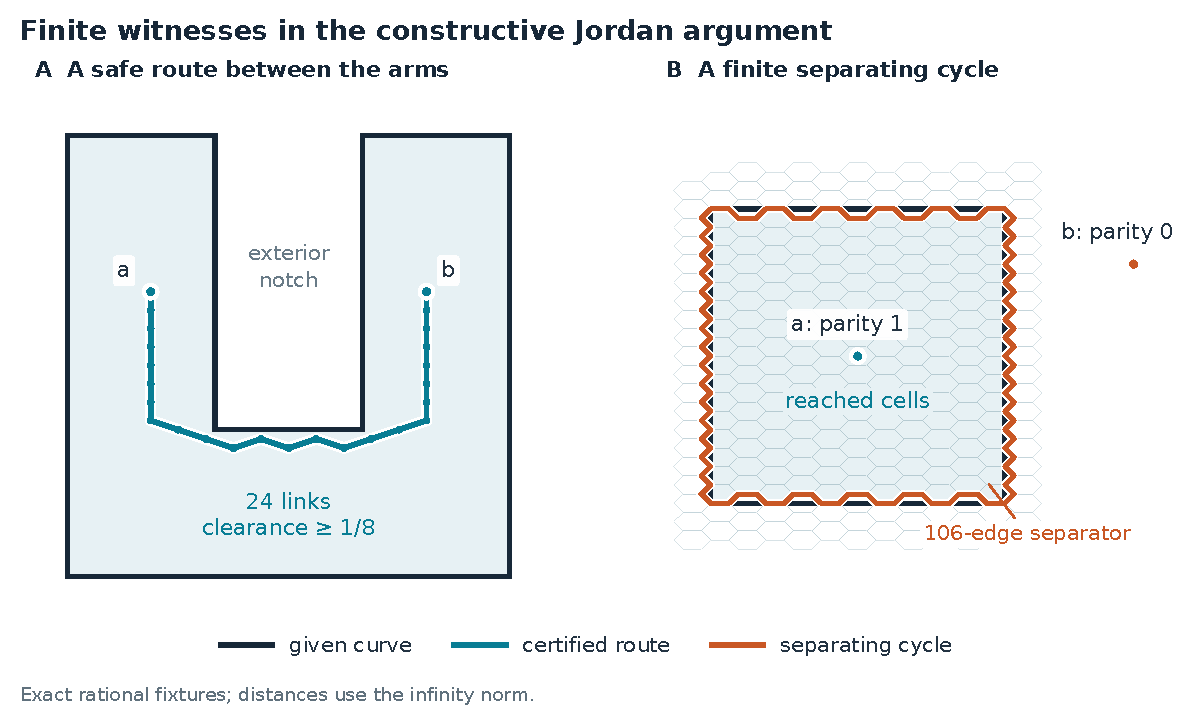
\includegraphics[width=\textwidth]{figures/finite_routes.pdf}
\caption{Exact finite examples from the accompanying kernel. Left:
a safe honeycomb route joins the two arms of a concave polygon;
its maximum-norm clearance is $1/8$. Right: flooding from a square's
interior leaves an exterior target unreached and produces a separating
cycle. These examples illustrate the finite constructions; the proof
above applies to the general named curve by the certified net test.}
\label{fig:routes}
\end{figure}

\section{Both sides at every curve point}\label{sec:boundary}

Routing alone would allow the possibility that every off-curve point
has bit zero. We must construct bit-one points, and we must do so
arbitrarily near every curve point. This is the remaining geometric
part of the theorem.

\subsection{A small rational square and two parameter half-arcs}

First let $t_0$ be rational modulo one, and write
\[
 c=\gamma(t_0),\qquad d=\gamma(t_0+1/2),\qquad
 D=2^{-V(1)}.
\]
The inverse separation assumption gives $\norm{c-d}\ge D$.
For a requested radius $2^{-n}$, put
\begin{equation}
 m=\max(n+4,V(1)+4,4),\qquad e=2^{-m},\qquad
 q=G(t_0,m+4).
 \label{eq:localsquare}
\end{equation}
The rational center $q$ satisfies $\norm{q-c}\le e/16$.
Let $Q$ be the boundary of the rational square
$q+[-e,e]^2$. We have
\begin{align}
 \dist(c,Q)&\ge15e/16,\label{eq:insideq}\\
 \dist(d,Q)&\ge D-17e/16\ge239e/16,\label{eq:outsideq}\\
 \norm{z-c}&\le17e/16<2^{-n}\quad(z\in Q).\label{eq:qnear}
\end{align}
The point $c$ is strictly inside this square; $d$ is strictly outside.
Thus
\begin{equation}
                      \parity(Q,c)=1,\qquad \parity(Q,d)=0.
 \label{eq:qvalues}
\end{equation}
These parities at named real points are calculated through rational
approximations using their displayed clearances.

Split the parameter circle into the two closed half-intervals with
endpoints $t_0,t_0+1/2$. Let their images be $A$ and $B$.
Each is a uniformly continuous path from $c$ to $d$,
with direction irrelevant to parity.
Set
\begin{equation}
 r=U(m+4),\qquad K=V(r),\qquad \eta=2^{-K}.
 \label{eq:localscale}
\end{equation}
Subdivide every side of $Q$ into
\begin{equation}
                     T=2^{K-m+7}
 \label{eq:Tsquare}
\end{equation}
equal segments. The exponent is nonnegative by the normalization
of the moduli, and every segment has length exactly $\eta/64$.
There are $4T$ segments, all specified before any color decision.

\subsection{A finite color test with a genuine overlap margin}

\begin{lemma}[The two half-arcs cannot both be close]\label{lem:arcs}
For each short square segment $E$,
\[
       \dist(E,A)<\eta/4\quad\Longrightarrow\quad
       \dist(E,B)\ge\eta/4.
\]
\end{lemma}

\begin{proof}
If a point $a\in A$ and a point $b\in B$ were each within
$\eta/4$ of $E$, then
\[
                  \norm{a-b}<\eta/4+\eta/64+\eta/4<\eta.
\]
For rational parameters the inverse condition forces their circular
distance below $2^{-r}$. Two parameters in opposite half-intervals
that are this close must both be within $2^{-r}$ of the same
endpoint, either $t_0$ or $t_0+1/2$. This is an interval calculation:
after translating $t_0$ to zero, the parameters lie in
$[0,1/2]$ and $[1/2,1]$, and the short gap is either across
$1/2$ or across $0=1$.
The forward modulus puts $a$ within $e/16$ of $c$ or $d$.
It follows that the square is within $e/16+\eta/4$ of that
endpoint, contradicting \eqref{eq:insideq} or \eqref{eq:outsideq}.

All positive closeness witnesses used in the algorithm come from
rational parameter samples. The conclusion for an arbitrary named
parameter follows by approximation. Equivalently, the weak lower
bound on the distance to $B$ means its rational approximations
satisfy the corresponding lower bounds at every precision.
If any such bound failed with positive slack, the preceding
finite rational contradiction would apply. No decision of
real equality or real trichotomy is involved.
\end{proof}

Approximate $\dist(E,A)$ by a rational number $D_E$ with error
at most $\eta/256$. To be explicit, use a mesh of the half-interval
with $2^{U(K+9)+1}$ subdivisions and evaluate at precision $K+9$.
Oscillation and evaluation together cost at most
$2\cdot2^{-(K+9)}=\eta/256$. Minimize the exact rational
point-to-segment distances as in Section~\ref{sec:nets}.
Color the segment by
\begin{equation}
 \begin{array}{lll}
 \text{red}&\text{if }D_E\ge\eta/8,&
       \dist(E,A)\ge31\eta/256>\eta/16,\\
 \text{blue}&\text{if }D_E<\eta/8,&
       \dist(E,B)\ge\eta/4.
 \end{array}
 \label{eq:squarecolors}
\end{equation}
For the blue case,
$\dist(E,A)<33\eta/256<\eta/4$, so
Lemma~\ref{lem:arcs} applies. The estimates leave a specified
rational gap on both branches.

A vertex common to segments of different colors has distance at least
$\eta/16$ from $A$ by its red segment, and at least $\eta/4$
from $B$ by its blue segment. It is therefore off the entire
curve with clearance at least $\eta/16$.

The coloring cannot be monochrome. If all segments were red,
the arc $A$ would be separated from $Q$ by $\eta/16$; if all
were blue, the arc $B$ would be separated from $Q$ by $\eta/4$.
In either case that arc joins $c$ to $d$ while avoiding the
closed walk $Q$, so Proposition~\ref{prop:stable} would give
$\parity(Q,c)=\parity(Q,d)$, contradicting \eqref{eq:qvalues}.
Since the $4T$ colors form a finite cyclic list, there are
at least two color-change vertices.

\subsection{The transition vertices cannot all have one curve bit}

List the transition vertices in cyclic order as
$w_0,\ldots,w_{s-1}$, and let $Q_j$ be the monochromatic
run from $w_j$ to $w_{j+1}$, with subscripts modulo $s$.
These are rational polygonal paths along the square, and their
concatenation is $Q$.
Each $w_j$ has the clearance $\eta/16$, so its curve bit is
a bounded calculation.

Suppose all these bits were equal. The connection theorem supplies
for each $j$ a rational polygonal route $P_j$ from $w_j$ to
$w_{j+1}$, with positive clearance from the entire curve.
Let $R$ be the closed walk obtained by concatenating all $P_j$,
and let $L_j$ be the closed walk following $P_j$ and then
the reverse of $Q_j$.

The walk $R$ avoids $A$, and $A$ joins $c$ to $d$; hence
\[
                         \parity(R,c)=\parity(R,d).
\]
If $Q_j$ is red, $L_j$ avoids $A$; if it is blue, $L_j$ avoids
$B$. In both cases the appropriate half-arc joins $c$ to $d$,
so
\[
                         \parity(L_j,c)=\parity(L_j,d).
\]
The finite chain identity modulo two is
\[
                         \sum_{j<s}L_j=R+Q.
\]
Taking parity at $c$ and at $d$, then xoring the preceding
equalities, forces $\parity(Q,c)=\parity(Q,d)$.
This again contradicts \eqref{eq:qvalues}.

The assertion that all transition bits are equal is decidable.
The contradiction therefore proves that a bounded scan of the
at most $4T$ vertices finds one with bit zero and one with bit one.
Both have clearance at least $\eta/16$ and both are within
$2^{-n}$ of $c$ by \eqref{eq:qnear}.
The auxiliary routes $P_j$ in the contradiction do not need to
stay in the small square or near $c$.

\begin{proposition}[Local witnesses with explicit bounds]\label{prop:local}
For rational $t_0$ and target precision $n$, the construction
\eqref{eq:localsquare}--\eqref{eq:Tsquare} returns rational
points of both curve bits, each within $2^{-n}$ of
$\gamma(t_0)$ and each with clearance at least
$2^{-K-4}=\eta/16$. Its candidate list has at most
$4\cdot2^{K-m+7}$ elements.
\end{proposition}

For a named parameter $t$, first take a rational parameter $t_0$
with $d_\T(t,t_0)\le2^{-U(n+2)}$. Such a parameter is obtained
by reading the parameter name at the specified precision.
Then $\norm{\gamma(t)-\gamma(t_0)}\le2^{-(n+2)}$.
Apply Proposition~\ref{prop:local} with target $n+2$ at
$t_0$. Its two outputs are within $2^{-(n+1)}<2^{-n}$ of
$\gamma(t)$. This proves the both-sides clause for arbitrary
named curve points without choosing an irrational split parameter.

\section{Completing the theorem}\label{sec:completion}

\subsection{The two regions and their sizes}

Define $I$ and $O$ to be the off-curve points with bits one and
zero, respectively. The classification calculation places every
off-curve point in exactly one of them. Local constancy makes
both quantitatively open: a point with clearance $r$ has a
ball of radius $r/4$ of its own bit. The connection theorem
joins any two points of either region by a positive-clearance
polygonal route. Conversely, Proposition~\ref{prop:stable}
prevents such a route between different regions.

If a closed polygonal walk lies in a convex box and the query is
outside that box, its parity is zero: join each edge to the first
vertex to form a triangle fan. Every triangle avoids the query,
and its two radial edges cancel with its neighbors.
Fine approximations of $\Gamma$ lie in the box used in
\eqref{eq:R}; hence every point outside that box has curve bit zero.
If the gap from the box is given by a positive rational number,
the required precision is specified by that gap.
For a merely asserted strict gap, instantiate its positive
rational witness; no unbounded search is required for the proof.

Thus $I\subset[-R,R]^2$. It is inhabited by
Proposition~\ref{prop:local} at $t_0=0$.
The points $(R+j+2,0)$, for $j\in\N$, have bit zero and
clearance at least $j+2$; this proves the asserted constructive
unboundedness of $O$. This also fixes the names: bit one is
inside and bit zero is outside.

\subsection{Approximate intersections of crossing paths}

Let a named uniformly continuous path $\alpha:[0,1]\to\R^2$
have endpoints of different bits, and fix $\eps=2^{-n}$.
Using its modulus and $U$, construct finite rational nets
$X_i$ and $Y_j$ for the path and the curve, respectively,
each with total net error at most $\eps/8$ and individual
evaluation error at most $\eps/8$. These nets include the
appropriate endpoint samples. Compute the rational number
\[
                         D=\min_{i,j}\norm{X_i-Y_j}.
\]
If $D\ge\eps/2$, then for arbitrary path and curve parameters,
the net estimates give distance at least
$D-\eps/8-\eps/8\ge\eps/4$.
The whole path would have positive clearance, contradicting
the endpoint bits and Proposition~\ref{prop:stable}.
The comparison is rational and decidable, so $D<\eps/2$.
A least minimizing pair of indices supplies rational parameters
$s_i,t_j$ with
\[
 \norm{\alpha(s_i)-\gamma(t_j)}
      \le D+\eps/8+\eps/8<3\eps/4<\eps.
\]
The algorithm has a completely specified finite product of meshes
as its search space. It proves approximate contact at each
requested precision. It does not choose an exact zero of a
continuous real function.

\subsection{The exact common-boundary converse by Cauchy names}
\label{sec:boundary-converse}

We have already constructed both bits in every neighborhood of every
curve point. For completeness, we prove the converse in the precise
positive-neighborhood sense stated in Theorem~\ref{thm:main}.
Suppose a named point $x$ has the property that, for every positive
dyadic radius, its neighborhood contains a \emph{rational}
off-curve point of each bit. More precisely, its arithmetic
premise is: for every $n$ there exist rational point codes
$a_0,a_1$ and natural clearance exponents $k_0,k_1$ such that
$\operatorname{Off}(a_i,k_i)$, $b_\Gamma(a_i)=i$, and
$\norm{a_i-x}<2^{-n}$. Strict closeness is expressed by a
finite precision witness in the name of $x$.
These are ordinary number-coded existential witnesses;
a separate choice sequence is not needed.

This rational formulation does not weaken the neighborhood
condition for named points. Given a named off-curve point,
approximate it rationally within a quarter of its positive
clearance and within a quarter of the remaining neighborhood
margin. Local constancy preserves its bit, and the approximation
has a positive clearance. Thus arbitrary named witnesses can
always be replaced by rational ones.

For any dyadic $\tau>0$, sample the curve and $x$ sufficiently
accurately that the combined net and query error is at most
$\tau/8$. Let $D$ be the minimum rational query-to-sample
distance. If $D\ge\tau/2$, every curve point is at least
$3\tau/8$ from $x$. Choose, from the neighborhood premise,
points of both bits within $\tau/16$ of $x$. The segment
joining them lies in that ball and has clearance at least
$3\tau/8-\tau/16>0$. Its endpoint bits must be equal,
a contradiction. Therefore $D<\tau/2$.
The bounded argmin returns a rational parameter $s(\tau)$ such that
\begin{equation}
                     \norm{\gamma(s(\tau))-x}<\tau.
 \label{eq:nearparameter}
\end{equation}
Notice that this parameter is computed just from the point and
curve names. The neighborhood premise is used to prove the
calculation succeeds, not to select an infinite family of data.

Now set
\[
 \tau_n=2^{-V(n+4)-3},\qquad t_n=s(\tau_n).
\]
For $j\ge n$, monotonicity of $V$ and \eqref{eq:nearparameter}
give
\[
 \norm{\gamma(t_j)-\gamma(t_n)}
    <\tau_j+\tau_n\le 2^{-V(n+4)-2}<2^{-V(n+4)}.
\]
The inverse condition, applied to the rational parameters,
therefore yields
\begin{equation}
                         d_\T(t_j,t_n)<2^{-(n+4)}.
 \label{eq:circlecauchy}
\end{equation}
This is already a primitive recursive fast name in the completed
parameter circle.

One may make it a conventional real Cauchy name explicitly.
Choose the representative $t_0\in[0,1)$ and put $z_0=t_0$.
For each $n$, select the unique member
\[
 \Delta_n\in\{t_{n+1}-t_n-1,\ t_{n+1}-t_n,\ t_{n+1}-t_n+1\}
\]
of absolute value below $1/4$, and set $z_{n+1}=z_n+\Delta_n$.
The choice is a three-way rational comparison justified by
\eqref{eq:circlecauchy}. Moreover
$|\Delta_n|<2^{-(n+4)}$, so
\[
              |z_j-z_n|\le\sum_{i=n}^{j-1}2^{-(i+4)}
                         <2^{-(n+3)}\qquad(j>n).
\]
Thus $z_n$ is an explicitly primitive recursive Cauchy name;
its residue modulo one has name $t_n$. Let $t$ denote this
circle name. Forward continuity makes $\gamma(t_n)$ converge
to $\gamma(t)$ with an explicit rate, while
\eqref{eq:nearparameter} makes it converge to $x$.
For any required error choose
$n\ge\max(U(k+2),k+2)$ and combine the two bounds.
They show $\gamma(t)=x$ in the equality-of-names sense.

This constructs a preimage without compactness, an infinite
subsequence selection, or an unbounded search. Consequently
\[
 \Gamma=\{x:\text{every neighborhood of }x
                    \text{ contains rational points of }I\text{ and }O\}.
\]
Together with the local constancy and both-sides results, this
is the asserted constructive common-boundary statement.
All parts of Theorem~\ref{thm:main} are now proved.

\section{Why this proof fits iPRA}\label{sec:arithmetic}

There are two distinct obligations. The output procedures must be
primitive recursive, and their correctness must be provable with the
induction permitted in iPRA. The first alone does not imply the
second. We give the bookkeeping for both.

\subsection{Coding and the exact logical form}

Use a signed-integer code, positive-denominator rational pairs,
and a primitive recursive pairing function. A list can be a length
together with iterated pairs; lookup is bounded iteration of the
projection. For lists whose entries are below $M$, one may instead
use base $M+1$ digits and a length. Lists of length at most $M$
then have a primitive recursive code bound, for example a pairing
of $M$ with $(M+1)^{M+1}$. Thus even a phrase quantifying over
all paths of length at most $M$ is a bounded arithmetic phrase
after this coding.

Rational arithmetic uses cross multiplication and signed arithmetic.
Normalization by a gcd is optional; equality can always be tested by
cross multiplication. If a total routine encounters an invalid code
or a zero denominator outside its intended domain, give it a fixed
default value. Correctness is conditional on the explicit domain
predicates. Division with remainder, bounded minimum, maximum,
finite xor, and finite sorting all have standard bounded-loop
definitions using primitive recursion.

Write $\Reg_G(\vec a)$ for the universal arithmetic presentation
conditions of Section~\ref{sec:names}, with the primitive recursive
definitions fixed. For fixed point names $X,Y$, write
$\operatorname{Off}(X,k)$ for the universal clearance formula
there. The classification is a numerical primitive recursive term
$\operatorname{Bit}(\vec a,\vec x,k)$.
The router is another such term that returns a tag, a finite route
code, the exponent $H$ of its clearance, and finite parent and
distance certificates. Its output terms have total default branches.
The useful assertion has the form
\begin{gather*}
 \Reg_G(\vec a)\wedge
 \operatorname{Off}(X,k_x)\wedge\operatorname{Off}(Y,k_y)
 \\[1mm]
 \longrightarrow\ \bigl(\operatorname{Bit}(X,k_x)=\operatorname{Bit}(Y,k_y)
       \\[-1mm]\hspace{18mm}\longrightarrow\
       \operatorname{RouteCorrect}
          (X,Y,\operatorname{Route}(X,Y,k_x,k_y))\bigr).
\end{gather*}
This is an ordinary first-order formula after expanding the
notations. A route's rational intermediate vertices are finite codes.
Its first and last vertices use the fixed input names.
Their segment interpolations are primitive recursive combinations
of these names and rational coefficients, rather than calls to an
interpreter for arbitrary programs.

The finite part of route correctness can be particularly concrete.
The stored curve net has error at most $h/8$, and every used
center link $S$ satisfies the rational check
\[
                \min_j\dist(S,Y_j)\ge3h/2.
\]
This finite check, the net correctness theorem, and the short-endpoint
inequalities imply the universal clearance conclusion. The output
does not consist merely of a search claim; its finite route and
the data certifying each link are the numerical witnesses.

For the local-boundary procedure the output is a pair of rational
point codes, two finite parity calculations, and the common
clearance exponent $K+4$. Its correctness is an analogous formula
from $\Reg_G$ to the two bit values, the dyadic distance bounds,
and the universal clearance assertions.

Uniformity is by substitution of fixed primitive recursive
definitions into these constructions. A family with additional
number parameters is still one schema instance. We make no
claim that validity of an arbitrary presentation is decidable,
or that iPRA proves the regularity premises of every true
presentation.

\subsection{Padding from rational conditions to completed names}
\label{sec:padding}

To remove a minor convention issue about endpoints of modulus
inequalities, one can begin with rational-parameter moduli
$U_0,V_0$ satisfying \eqref{eq:arithU}--\eqref{eq:arithV}
on rational parameters. Normalize them by finite maxima.
For the completed names use the more generous moduli
\begin{equation}
        U(k)=U_0(k+2)+2,\qquad V(k)=V_0(k+2)+2,
 \label{eq:padded}
\end{equation}
and normalize again if needed.

For example, if completed parameters have distance
at most $2^{-U(k)}$, sufficiently accurate rational approximations
have distance strictly below $2^{-U_0(k+2)}$. Their images
are within $2^{-(k+2)}$ up to the specified approximation
errors, hence within $2^{-k}$ in the limit-name inequalities.
If the completed parameters have distance at least $2^{-k}$,
their sufficiently accurate rational approximations have distance
at least $2^{-(k+2)}$. Their image separation is at least
$2^{-V_0(k+2)}$ up to arbitrarily small errors, and therefore
at least $2^{-V(k)}$.

This passage is an estimate at each requested precision.
It is not an application of compactness or of real-number
trichotomy. All the proof's named constants refer to the padded
$U,V$ if the input was originally given only in rational form.

Evaluation on a completed parameter is explicit as well.
If $q_j$ is a fixed fast circle name for $t$ with
$d_\T(q_j,t)\le2^{-j}$, use
\[
                    G(q_{U(k+2)},k+2)
\]
as an approximation to $\gamma(t)$ at target precision $k$.
Forward continuity and evaluation contribute at most
$2^{-(k+2)}$ each. This is a primitive recursive composition
for the fixed name; an unnamed extension operator is unnecessary.

\subsection{An explicit bound ledger}
\label{sec:bounds}

The following are deliberately generous bounds. They are intended
to demonstrate primitive recursiveness, not practical efficiency.
Let the routing parameters be those of
\eqref{eq:route-scale}--\eqref{eq:board}, and put
$N=2^{U(H+4)+1}$.

\begin{center}
\begin{tabular}{@{}p{0.59\textwidth}p{0.33\textwidth}@{}}
\toprule
Operation & A priori bound\\
\midrule
Curve samples used for link tests & $N$\\
Rational point-to-segment minimization & at most $8$ candidates\\
Board cells & $M=(2L+1)^2$\\
Neighbor-link tests, allowing duplicates & $6M$\\
Reachability propagation & $M$ rounds\\
Parent route in the board & $M-1$ links\\
Route with original endpoint connectors & $M+1$ segments\\
Separating-cycle trace & $6M$ edges\\
Expanded cyclic-mesh walk in factorization & $6MN$ edges\\
Edge-usage bit table & $N$ entries\\
\bottomrule
\end{tabular}
\end{center}

A direct implementation can use $M$ rounds, each scanning all
$M$ cells and six neighbors. This gives at most $6M^2$
Boolean propagation tests after the geometric link table has
been calculated. A queue implementation improves this bound,
but the proof does not need the improvement.
The shortest-coordinate path used to find a separating edge
has at most $4L$ links.

For the local-square argument, use $m,K,T$ from
\eqref{eq:localsquare}--\eqref{eq:Tsquare}. There are
$4T$ segments and no more than $4T$ transition vertices.
One half-arc net with at most
$2^{U(K+9)+1}+1$ samples is sufficient for all color tests.
Every transition vertex has clearance $2^{-(K+4)}$,
so the hypothetical same-bit routes in the contradiction
can all use
\[
 k_{\mathrm{local}}=K+7,\qquad
 H_{\mathrm{local}}=V(U(K+11))+10
\]
and a common board based, for example, on $B=R+8$.
All square vertices have norm below $R+1$ with the generous
bound \eqref{eq:R}. Thus the finite family of at most $4T$
auxiliary route calculations also has a displayed primitive
recursive bound. The witness-finding procedure itself only
needs to compute the transition bits and select the two values.

For approximate intersection at precision $n$, one may use
$2^{W(n+4)+1}+1$ path samples, where $W$ is the path's forward
modulus, and $2^{U(n+4)+1}$ curve samples. The product of
these two finite numbers bounds the pair search.

Every function in this ledger is obtained from supplied fixed
primitive recursive functions by composition, arithmetic,
exponentiation, finite maxima, and bounded iteration. A call
to $U$ or $V$ at a computed argument is just composition.
No step increases its precision until some undecidable
condition happens to become true.

\subsection{Quantifier-free induction, step by step}
\label{sec:qfind}

For a primitive recursive Boolean predicate $A(i,\vec z)$, define its
Boolean fold
\[
 C_A(0,\vec z)=1,\qquad
 C_A(s+1,\vec z)=
     C_A(s,\vec z)\,[A(s,\vec z)].
\]
The finite universal statement
$\forall i<s\,A(i,\vec z)$ is represented by the equation
$C_A(s,\vec z)=1$. Finite existential statements use the
corresponding or-fold; least witnesses are bounded scans.
Hence the induction invariants below are quantifier-free
equations or Boolean combinations of equations in the
language containing the relevant primitive recursive functions.

\begin{longtable}{@{}p{0.24\textwidth}p{0.69\textwidth}@{}}
\toprule
Construction & Induction invariant and step justification\\
\midrule
\endhead
Finite minima &
The stored candidate is among the processed candidates and has
value no larger than each of them. The new candidate is compared
by decidable rational order. A bounded fold records all preceding
comparisons.\\[3pt]
Ray parity &
The accumulator is the xor of the processed edge contributions.
For a triangle the calculation is a fixed finite case analysis;
for a list of triangles, adding the next triangle cancels its
twice-occurring internal edges.\\[3pt]
Mesh refinement &
The current edge chain is the original chain plus the boundaries
of the triangles already inserted. Each new triangle has its
specified margin from the query, so its parity is zero.\\[3pt]
Reachability &
Every discovered cell has a recorded safe path of length at
most the current round. After round $s$, every safe path of at
most $s$ links ends in the reached set. Path codes of these
lengths have an explicit finite bound.\\[3pt]
Parent extraction &
The current parent has strictly smaller discovery rank.
Each chosen parent link is safe and the current reversed list
has no repeated cell. At most $M$ parent lookups suffice.\\[3pt]
Stabilization &
If a reached set has not stabilized, the next round adds a
new cell. A bounded count of distinct reached cells increases
and cannot exceed $M$. Equivalently, bounded loop deletion
shortens every walk to at most $M-1$ links.\\[3pt]
Boundary traversal &
Orient separating edges with green on the left. This table has
one successor and one predecessor at each used vertex. Its current orbit has no
repetition before its return. The local degree statement is
the eight-case calculation for three cell colors.\\[3pt]
Cycle factorization &
At each sample vertex, the xor of the two incident usage bits
is zero. Induction on the cyclic vertex index makes every
usage bit equal to the initial one. The total parity is the
corresponding finite xor identity.\\[3pt]
Square contradiction &
After $j$ monochromatic runs, the xor of the $j$ loop chains
equals the xor of their routes and their square runs.
The equalities at $c,d$ telescope by adding one run.\\[3pt]
Circle-name lift &
After $j$ increments the lift projects to the selected
circle residue, and the absolute accumulated increment is
bounded by the finite geometric sum. Its bound is proved
by rational arithmetic induction.\\
\bottomrule
\end{longtable}

Some invariants are naturally first expressed as bounded
quantification over arrays or lists. The fold translation just
described is part of the proof, so those do not become new
unbounded induction instances. The natural induction counters
are list lengths, board rounds, or positions in finite sums.

The universal presentation hypotheses remain assumptions in
the deduction context. During a step they are instantiated at
the rational parameters and precisions occurring in that step.
Safe-edge and replacement-triangle margins are recorded as finite
rational certificate predicates. Induction verifies those
predicates; the general net lemma then gives the universal
clearance conclusion with an arbitrary curve parameter held fixed.
One does not induct on the unbounded assertion that all
previous paths avoid the named curve.
We do not induct on the assertion that a real-valued function
is continuous, that an arbitrary point belongs to a component,
or that a formula holds for every real point. For a geometric
estimate with an arbitrary query or precision, hold those
number parameters fixed, perform the finite calculation and
its quantifier-free induction, and generalize afterward.

This also explains why the exact common-boundary converse does
not require stronger induction. For fixed $n,j$ the closeness
of the two selected parameters follows directly from their
two distance bounds and the separation condition. Only the
finite sum of lifted increments uses induction, and its
invariant is a rational inequality.

\subsection{Where intuitionistic reasoning matters}

The proof uses case distinctions only on coded rational
comparisons, finite lists, or bits. In the routing argument,
reachability is one such finite Boolean value. In the local
square argument, the assertions that all segment colors agree
and that all transition bits agree are finite Boolean tests.
In the approximate intersection and boundary converse,
the test $D\ge\eps/2$ is a rational comparison.
Showing one branch contradictory therefore permits selection
of the other branch intuitionistically.

The use of a positive inverse modulus is also precise.
Given two rational parameters, compare their distance with
$2^{-r}$. The greater-or-equal case contradicts the
strictly smaller image-distance estimate, so the strict
parameter-distance bound follows. This is not the
contrapositive of mere negative injectivity.

We have used neither unrestricted excluded middle nor
Markov's principle, neither a fan theorem nor weak
K\"onig's lemma, and neither a general extremum theorem
nor an intermediate value selection principle.
The completed-name language packages explicit rational
estimates; it is not an additional axiom asserting the
existence of arbitrary infinite objects.

\begin{corollary}[First-order iPRA reading]\label{cor:ipra}
For every fixed tuple of primitive recursive definitions
for the presentation and any required point and path names,
the arithmetic versions of Theorem~\ref{thm:main} are
derivable in intuitionistic primitive recursive arithmetic.
Their witness procedures are the primitive recursive
constructions above. The derivations are conditional on
the stated arithmetic regularity and clearance premises.
\end{corollary}

\begin{proof}
Introduce the finitely many required primitive recursive
function symbols with their defining equations. Prove the
bounded arithmetic and finite geometry lemmas by the
quantifier-free invariants just listed. Substitute them
into the proofs of Sections~\ref{sec:parity}--\ref{sec:completion}.
All other logical steps are first-order intuitionistic
introduction and elimination rules. Existential output
claims are introduced with the already specified witness
terms. The arbitrary requested precision is then universally
generalized. The construction uses exactly the defining
equations and quantifier-free induction available in iPRA.
\end{proof}

This corollary is a human proof of formalizability with an
explicit induction audit. It is not a claim that the many
object-theory proof terms have already been generated and
checked by Lean. The next section identifies that remaining
mechanical task and the exact existing repository interface.

\section{Lean formalization: a concrete completion route}\label{sec:lean}

\subsection{What can be reused from ProveIt}

The repository was inspected at the immutable commit
\[
 \texttt{620f5e3b959c3a4284060ada5efb651812612319}.
\]
Its root toolchain specifies Lean \texttt{v4.32.0} and the
matching Mathlib tag. The relevant existing development is
\texttt{Logic/PrimitiveRecursiveArithmetic/ConciseIPRA}.
The following are actual declarations in the inspected sources
\cite{ProveIt}, not proposed names.

\begin{center}
\begin{tabular}{@{}p{0.38\textwidth}p{0.54\textwidth}@{}}
\toprule
Existing interface & Use in this project\\
\midrule
\code{PR}, \code{PTm} in \code{PR.lean} &
Primitive recursive function symbols and first-order terms.
The constructors of \code{PR} are zero, successor,
projection, composition, and primitive recursion.\\[3pt]
\code{PRAAx} &
Defining equations, successor nonzero and injectivity,
and the quantifier-free induction schema.\\[3pt]
\code{PRA.qfInd} &
Build an object-level induction derivation from a QF formula
and derivations of its base and successor cases.\\[3pt]
\code{Prf} in \code{Deduction.lean} &
The intuitionistic first-order derivation type.\\[3pt]
\code{NFm.ofPRA}, \code{pra\_iff\_native} &
Translate a completed iPRA derivation into the native
ConciseIPRA calculus.\\
\bottomrule
\end{tabular}
\end{center}

The repository's native/scalar equivalence does not automatically
turn a Mathlib theorem about real curves into an iPRA derivation.
Its use here is precise: after constructing the arithmetic
derivation, apply the existing theorem
\[
 (\Gamma\vdash[\mathsf{PRAAx}]\varphi)
   \ \longleftrightarrow\
 \mathsf{NPrf}\,(\Gamma.\mathsf{map}\,\mathsf{NFm.ofPRA})\,
                   (\mathsf{NFm.ofPRA}\,\varphi).
\]
The accompanying \code{NativeTransfer.lean} contains exactly
this generic wrapper with the real repository API.

The supplied draft directory was inspected for context. It contains
other constructive-analysis archives, but this proof needs none
of their claimed analytic results. In particular there is no
dependency on a formalized fundamental theorem of algebra,
an integral winding number, or an existing Jordan theorem.

\subsection{Three deliverable layers}

The completion should keep three layers distinct.

\begin{enumerate}
\item \textbf{Executable finite mathematics.}
Define rational points, half-open ray parity, meshes, distance
certificates, the finite honeycomb, reachability, boundary
traversal, and the numerical procedures from the bound ledger.
The Python implementation is a reference for this layer.
\item \textbf{Lean semantic verification.}
Prove the finite algorithms correct for their explicit data
structures. Named-curve theorems can then be stated using
fast Cauchy names, supplied moduli, and finite certificates.
This checks the mathematical construction.
\item \textbf{Object-level iPRA derivations.}
Represent the finite routines by \code{PR} expressions,
their Boolean invariants by equations of \code{PTm}, and
their proofs by \code{Prf PRAAx}. Use \code{PRA.qfInd}
for every loop invariant. Finally translate with
\code{pra\_iff\_native}.
\end{enumerate}

A proof in layer 2 alone is not a substitute for layer 3.
Conversely, once layer 3 produces a derivation in the explicit
intuitionistic calculus, a general analytic theorem from Mathlib
is unnecessary as a trusted premise.

\subsection{Module order and exact proof obligations}

\begin{longtable}{@{}p{0.20\textwidth}p{0.73\textwidth}@{}}
\toprule
Proposed module & Required results\\
\midrule
\endhead
\code{Coding} &
Integer/rational/list codes, bounded folds and scans, finite
minimum, powers and moduli composition. Supply \code{PR}
terms and defining-equation proofs.\\[3pt]
\code{Geometry} &
Rational segment membership and intersections; the
at-most-eight-candidate maximum-norm distance algorithm;
convex-combination norm inequalities.\\[3pt]
\code{Parity} &
The half-open edge test, xor additivity, reversal,
triangle parity outside its hull, convex-square and
parallelogram values. All cases are rational sign cases.\\[3pt]
\code{Replacement} &
Finite triangle-boundary cancellation, query-translation
parallelograms, mesh refinement, and stable curve parity
with explicit rational-margin certificates.\\[3pt]
\code{CycleWalk} &
Short-arc selection in a cyclic array; usage-bit incidence
at each vertex; constancy of all edge-usage bits;
Lemma~\ref{lem:factor} with the bound $sN$.\\[3pt]
\code{Honeycomb} &
The six vertices and neighbor table, vertical-slice
coverage, shared-edge identities, three-cell vertices,
and the center-link crossing and detour calculations.\\[3pt]
\code{FiniteGraph} &
$M$-round reachability, parent paths, stabilization,
monochromatic outer ring, degree-two cycle extraction
with at most $6M$ steps.\\[3pt]
\code{Connection} &
Near/safe link certificates; cycle proximity; local
parity jump; product-bit contradiction; route validity
and clearance at least $h$.\\[3pt]
\code{BothSides} &
The local square, half-arc nets, color certificates,
transition clearance, and the finite chain contradiction.
Produce rational witnesses with clearance $2^{-K-4}$.\\[3pt]
\code{Names} &
Cauchy names, padded moduli, finite distance nets,
completed evaluation, and the explicit circle-name lift.
Universal estimates are derived after finite certificates.\\[3pt]
\code{JordanSchema} &
Classification, route theorem, both-sides theorem,
size bounds, approximate intersection, and the
rational-witness common-boundary characterization.\\[3pt]
\code{NativeJordan} &
Assemble the closed arithmetic formulas and object-level
proofs; apply the existing native translation.\\
\bottomrule
\end{longtable}

The practical first milestone is \code{Parity} plus
\code{FiniteGraph}. It isolates the finite proof without
introducing a real-number library. The next milestone is
the factorization and routing theorem for finite sample
certificates. Only afterward should the names and moduli
interface connect those certificates to continuous curves.

There is no unknown topological lemma left in this plan.
The substantial work is formalizing the stated rational sign
lemmas, array invariants, and their object-theory derivations.

\subsection{Suggested statement and derivation interfaces}

The semantic layer should make certificates explicit. Suitable
structures include the following fields (this is an interface
specification, not a claim that these complete structures have
already been implemented).

\begin{description}[leftmargin=0pt,labelindent=0pt]
\item[\texttt{CurvePresentation}]
Fixed rational approximation routines, $U,V$, and the
arithmetic Cauchy/continuity/separation predicates.
\item[\texttt{OffCertificate}]
A dyadic clearance exponent and the corresponding
universal rational-name inequalities.
\item[\texttt{NetCertificate}]
The finite sample list, its parameter mesh and evaluation
precision, and the rational constants in its error bound.
\item[\texttt{RouteCertificate}]
Finite rational intermediate vertices, parent indices,
safe-link checks against a certified net, and a dyadic
clearance exponent.
\item[\texttt{BoundaryWitnesses}]
Two rational points, their clearance exponents, their
finite bit calculations, and finite precision witnesses
to the requested proximity.
\end{description}

The statement for routing should return actual data, for example
a route certificate satisfying the endpoint and clearance
predicates, rather than only a proposition asserting that two
points are in one connected component. The approximate crossing
statement should return the two rational sample parameters.
The reverse-boundary statement should return the displayed
primitive recursive circle-name construction.

For object-level proof assembly, the recurring pattern is:
\begin{enumerate}
\item Express a finite invariant as a Boolean equation
$I(s,\vec z)=1$, where $I$ is a fixed \code{PR} expression.
\item Prove its zero equation from the defining equations.
\item From $I(s,\vec z)=1$, prove $I(s+1,\vec z)=1$ using
the rational sign lemmas and Boolean equations.
\item Apply \code{PRA.qfInd}; only then introduce the
desired universal quantifiers or replace a Boolean fold
by its bounded mathematical reading.
\end{enumerate}
The final target is an actual object-level value of the schematic
type
\begin{lstlisting}
[] |- [PRAAx] jordanSentence
\end{lstlisting}
with the repository's notation and all the primitive recursive
witness terms substituted. Here \code{jordanSentence} is a
project-specific encoded sentence to be defined; the line is
not a completed declaration in this archive.
The supplied native wrapper takes such a derivation as an input.

The semantic definitions and the \code{PR} expressions should
be connected by evaluation lemmas. This prevents a discrepancy
between the executable reference algorithm and the routine
whose correctness is proved inside iPRA. A small library of
verified constructors for bounded scans and array iterations
will amortize most of the proof-term bookkeeping.

\subsection{Verification gates and honest status}

For a completed formalization:
\begin{enumerate}
\item Build against the pinned repository toolchain, then run
\code{lake env lean} on each module and the library build.
\item Check the semantic finite lemmas on the same exact
fixtures as the Python reference.
\item Audit every induction formula used in the object
derivations and inspect the generated \code{PR} expressions.
\item Inspect \code{\#print axioms} for the final semantic
and proof-construction theorems, and inspect their imports.
An object-level derivation of the specified arithmetic
sentence is the final iPRA gate.
\end{enumerate}

The environment used for this package did not contain Lean.
The files \code{lean/FiniteKernel.lean} and
\code{lean/NativeTransfer.lean} are therefore explicitly marked
\emph{uncompiled scaffolds}. They contain executable definitions
and a generic existing-API transfer wrapper, no added
\code{axiom} declarations and no \code{sorry} proofs.
They do not state that Jordan's theorem has already been
machine-checked. The complete dependency and invariant plan
is also in \code{lean/ROADMAP.md}.

\section{Executable artifacts and reproducibility}\label{sec:artifacts}

The archive includes an exact rational finite kernel, tests, and
machine-readable results. Its geometry uses Python's
\code{fractions.Fraction}; no floating-point tolerances occur in
the assertions. Plotting converts coordinates to floating point
only after the exact checks.

The kernel implements:
\begin{itemize}
\item the half-open ray index and its parity;
\item exact rational segment intersections and maximum-norm
clearances;
\item the rational honeycomb and bounded flood fill;
\item finite parent routes and separating cycles;
\item cyclic-mesh labeling and both integer and mod-two
factorization checks.
\end{itemize}
The signed integer index is an optional stronger helper in the
reference program. The proof in this article only trusts the
parity calculation.

The delivered run passed \textbf{142 exact checks}. Its concrete
connection examples are:

\begin{center}
\begin{tabular}{@{}p{0.47\textwidth}p{0.17\textwidth}rr@{}}
\toprule
Example & Outcome & Segments & Clearance\\
\midrule
Square: inside to inside & route & 3 & $11/8$\\
Square: inside to outside & bits $1,0$ & -- & --\\
Concave U: one arm to the other & route & 24 & $1/8$\\
Concave U: notch to far exterior & route & 25 & $3/16$\\
\bottomrule
\end{tabular}
\end{center}

The square separator has 106 edges. An additional annular
cell-coloring fixture produces two separating cycles, with
54 and 18 edges. This checks a particularly relevant case:
the finite boundary need not be a single cycle.
Other assertions cover vertex-height degeneracies, collinear
subdivision, reversal, repeated traversal, affine coordinate
changes, triangle replacement, all six neighbor identities,
and cyclic-mesh parity multiplication.

These checks validate the executable finite examples. They
are not an exhaustive check of the general theorem or a
substitute for its proof, and the reference implementation
uses polygons as finite distance oracles. The paper supplies
the certified net replacement for a general curve. The
Python program is not advertised as a completed extraction
of every continuous-name procedure in the paper.

To reproduce the finite checks and figures from the archive root:
\begin{lstlisting}
python3 artifacts/test_kernel.py
python3 artifacts/make_figures.py
\end{lstlisting}
The tests use only the Python standard library. The figure
script additionally needs Matplotlib. To compile the article:
\begin{lstlisting}
latexmk -pdf -interaction=nonstopmode -halt-on-error jordan_ipra.tex
\end{lstlisting}
All textual proof sections and the vector figure are included.
The README records the file layout and the verification
status in one place.

\clearpage
\begin{thebibliography}{9}
\bibitem{BJMR}
G. Berg, W. Julian, R. Mines, and F. Richman,
\emph{The constructive Jordan curve theorem},
Rocky Mountain Journal of Mathematics \textbf{5} (1975), 225--236.
\href{https://doi.org/10.1216/RMJ-1975-5-2-225}{doi:10.1216/RMJ-1975-5-2-225}.
Primary-paper text inspected through
\url{https://paperzz.com/doc/6807670/the-constructive-jordan-curve-theorem}.

\bibitem{NC}
P. Nguyen and S. Cook,
\emph{The Complexity of Proving the Discrete Jordan Curve Theorem},
\href{https://arxiv.org/abs/1002.2954}{arXiv:1002.2954} (2010).

\bibitem{Bridges}
D. S. Bridges,
\emph{On the Constructive Theory of Jordan Curves},
\href{https://arxiv.org/abs/2502.09784}{arXiv:2502.09784} (2025).

\bibitem{ProveIt}
V. Reshetnikov, \emph{ProveIt}, repository snapshot\\
\texttt{620f5e3b959c3a4284060ada5efb651812612319}, inspected
15 November 2026.
\url{https://github.com/VladimirReshetnikov/ProveIt}.
In \path{Logic/PrimitiveRecursiveArithmetic/ConciseIPRA/Lean/ConciseIPRA/},
the files \texttt{PR.lean}, \texttt{Deduction.lean}, and
\texttt{NativeBiInterpretation.lean} specify the arithmetic calculus and
the translation used in Section~\ref{sec:lean}.

\bibitem{JCT}
\emph{Jordan curve theorem}, the statement identified in the request,
\url{https://en.wikipedia.org/wiki/Jordan_curve_theorem},
accessed 15 November 2026.
This is used to identify the classical target, not as a proof dependency.
\end{thebibliography}
\end{document}
